\subsection{Domain-Service}
\label{subsec:implementation:domainService} 
Die gesamte Geschäftslogik, wie das Verhalten von Flügen, Tickets und anderen Entitäten, wird in der Komponente \textit{Domain-Service}  abgebildet. Die Actoren welche sich in dieser Komponente befinden, wurden so abgebildet, dass die Repräsentation der Anwendung selbst keine Rolle spielt. Das bedeutet, dass die Implementierung in dieser Komponente unabhängig davon umgesetzt wurde, ob die Anwendung selbst über beispielsweise über das \textit{CQRS}-Prinzip verfügt oder ob die Interaktion mit dem Benutzer über eine \textit{HTTP} Schnittstelle umgesetzt wurde. \\
Die hier repräsentierten Entitäten, welche selbst ja wieder als Actoren implementiert wurden, beinhalten neben der eigenen Logik auch einen Zustand welcher Persistiert wird. Dies wird durch \textit{Event Soucing} ermöglicht, welches in Abschnitt \ref{subsec:implementation:eventSouring} genauer beschrieben wird. Ereignisse welche in der Entität selbst auftretten, werden persistiert und bei einem späteren Neustart des dazugehörigen Actors wieder eingespielt. Mit diesem Prinzip sind alle nachfolgend beschriebenen Entitäten ausgestattet. \\
Um eine Verteilung der Entitäten zu ermöglichen, werden diese in Form von \textit{Sharding} auf unterschiedliche Hosts verteilt. \textit{Sharding} selbst wird in Kapitel \ref{subsec:implementation:ApplicationDistribution} genauer betrachtet. Für eine Verteilung mittels \textit{Sharding} müssen Actoren bestimmt werden, welche anschließend verteilt werden. Alle Kindelement dieser Actoren werden anschließend an den gleichen Ort wie ihre Parents verschoben. Innerhalb des \textit{Domain Service} gibt es folgende Actoren welche durch \textit{Sharding} erteilt werden:
\begin{itemize}
    \item Flug Nummer (\textit{FlightNumber})
    \item Flug Ticket (\textit{FlightTicket})
    \item Buchungskoordinator (\textit{ChargingCoordinator})
\end{itemize}
Auf die genaue Aufgabe sowie die Implementierung dieser drei Actoren wird nun nachfolgend eingegangen.

\subsubsection{Flug Nummer}
Die Repräsentation der angebotenen Flüge selbst wird mit dem Actor \textit{FlightNumber} umgesetzt. Dieser beinhaltet Informationen über Start- und Zielort und den Zeitraum an welchem der Flug zur verfügung steht. Für Informationen über einen Flug an einem bestimmten Datum, wird ein neuer Actor herangezogen, welcher den operativen Flug darstellt. Der Actor \textit{OperateFlight} verwaltet Informationen über den Typ des Flugzeuges sowie der Passagierkapazität welche für diesen Flug angeboten wird. Informationen über Passagiere für den Flug werden jedoch nicht über den Actor selber verwaltet sondern an einen weiteren Actor, den \textit{FlightPassengerList}-Actor, welcher für diese Aufgabe spezialisiert ist, weitergereicht. \\
Der Actor \textit{FlightPassengerList} verwaltet für einen operativen Flug die verfügbaren Plätze. Dabei wird ihm, wie aus Abbildung \ref{fig:implementation:entityFlightNumber} zu entnehmen ist, von seinem \textit{Parent} dem \textit{OperateFlight}, die verfügbare Kapazität abhängig vom verwendeten Flugzeugtyp, mitgeteilt. Der Actor verwaltet nun eine Liste mit reservierten sowie bereits gebuchten Ticket für diesen Flug. Die Tickets selbst werden wiederum in einem eigenen Actor repräsentiert. Dieser gehört jedoch nicht mehr in die Hierarchie der Flugnummer, sondern befindet sich in einer eigenen, über \textit{Sharding} verteilten, Entität. \\
Nachrichten von ausserhalb dieser Hierarchie werden immer an den betreffenden \textit{FlightNumber} gesendet. Dieser leitetet die Nachricht weiter an den betroffenen \textit{OperateFlight} Actor, was nur möglich ist wenn die Nachricht auch die Informationen entsprechend bereitstellt. \\
Wird nun von einem \textit{CommandHandler} an den \textit{FlightNumber}-Actor der Befehl gesendet, ein Ticket zu reservieren, so wird dieser Befehl bis an die Passagierliste weitergereicht. Dort wird überprüft ob die Kapazitäten für eine neue Reservierung noch vorhanden sind. Ist dies der Fall, wird dieser Platz in der Passagierliste reserviert und ein neues Ticket erstellt. 
\begin{figure}
    \centering
    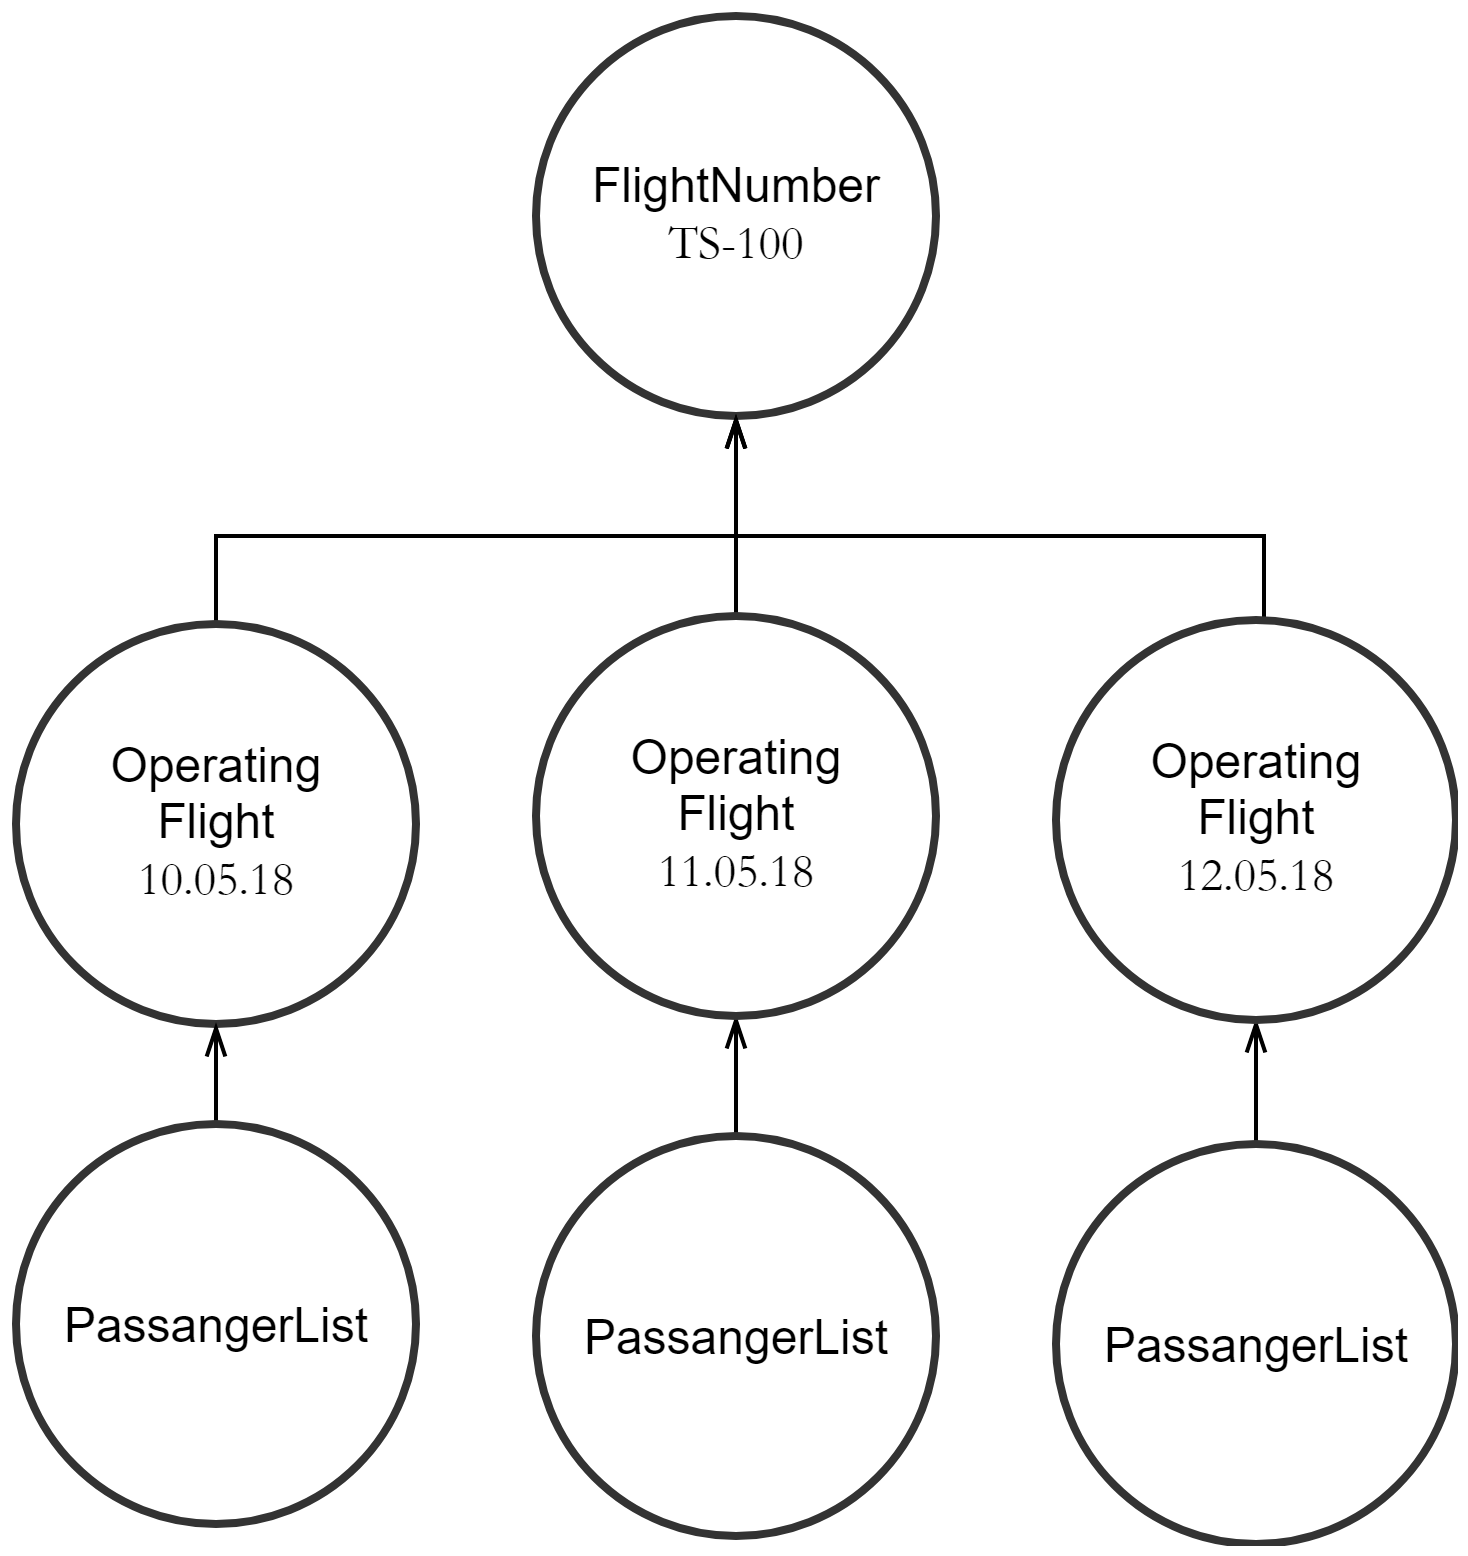
\includegraphics[width=0.65\linewidth]{gfx/implementation/FlightNumberSample}
    \caption{Darstellung eines Fluges welcher für drei Tage verfügbar ist.}
    \label{fig:implementation:entityFlightNumber}
\end{figure} 

\subsubsection{Flight Ticket}
Entscheidet ein \textit{PassangerList}-Actor ein neues Ticket für einen Flug zu erstellen, so wird dieses Ticket als neue Entität im \textit{FlightTicket} Sharding erzeugt. \\
Die Entität selbst repräsentiert eine Ticketreservierung welche eine eindeutige Ticketidentifikation besitzt. Über diese Identifikation kann jedes Ticket exakt angesprochen werden. Ein Ticket repräsentiert neben dem Inhaber des Tickets auch der aktuelle Ticketstatus. Jedes Ticket kann sich in einem der folgenden Zustände befinden:
\begin{enumerate}
    \litem{Reserviert} Das Ticket wurde Reserviert und der Platz im Flugzeug ist bis auf weiteres durch dieses Ticket blockiert. Wird nach einer konfigurierten Zeit kein Zustandswechsel der Ticketreservierung vollzogen, so storniert sich das Ticket selbstständig und der Platz wird wieder freigegeben.
    \litem{Gebucht} Der Bezahlvorgang für dieses Ticket konnte erfolgreich abgeschlossen werden und der gebuchte Sitzplatz bleibt ohne Zeitablauf für dieses Ticket reserviert.
    \litem{Stoniert} Das Ticket wurde entweder vom Benutzer selbst storniert. Weiters ist es möglich, dass der Bezahlvorgang nicht erfolgeich durchgeführt werden konnte oder sich das Ticket durch ablaufen eines Zeitfensters selbst storniert hat. Der reservierte Platz steht wieder für neue Reservierungen zur verfügung.
    \litem{Bezahlvorgang läuft} Wird ein Ticket gebucht so wird dadurch der Bezahlvorgang gestartet. Während dieser ausgeführt wird, befindet sich die Reservierung in diesem Status. Verläuft der Bezahlvorgang erfolgreich wird das Ticket in den Status \textit{Gebucht} wechseln, ansonsten in den Status \textit{Stoniert}.
\end{enumerate}
Für die Implementierung eines Zeitfensters für den Abblauf eines Tickets wird bei der Reservierung des Tickets eine Nachricht geplant. Das bedeutet, es wird zu Beginn der Reservierung vom Ticket selbst eine Nachricht an sich selbst versendet, welche signalisiert, dass ein Zeitfenster abgelaufen ist. Jedoch wird dabei beim versenden mittels dem \textit{Akka.Net} Framework eine Zustellzeit angegeben. Die Zustellung zum Actor wird dadurch verzögert. Wird die Nachricht zugestellt, kann der Actor selber entscheiden ob sie noch relevant ist. Ist beispielsweiße das Ticket mittlerweile in einem Zustand in welchem eine Stornierung nicht mehr notwendig ist, kann die Nachricht vom Actor verworfen werden, ansonsten kann die Stornierung der Reservation gestartet werden. \\
Der Bezahlprozess für die Buchung eines Tickets wird einem Koordinator übergeben welche die Buchung durchführt. Der \textit{FlightTicket}-Actor erhält von diesem Koordinator nach dem Bezahlvorgang eine Nachricht über den Ausgang des Bezahlprozesses und ändert anschließend den Zustand des Tickets entsprechend.

\subsubsection{Buchungskoordinator}
\label{subsub:implementation:ChargingCoordinator}
Wird ein bereits reserviertes Ticket gebucht, so erzeugt der Ticket-Actor für den Bezahlvorgang einen neuen Buchungskoordinator. Dieser Buchungskoordinator bekommt eine eigene Buchungs-Identifikation vom Ticket zugewissen. Der Buchungskoordinator selbst wird, wie auch die zuvor beschriebenen Entitäten, über \textit{Sharding} verteilt. Somit kann ein Ticket und der dazugehörige Buchungskoordinator auf unterschiedlichen Hosts instanziiert werden. \\
Die Aufgabe des Buchungskoordinator ist es, den gewünschten Betrag von einer externen Bankenschnittstelle abzubuchen. Die Bankenschnittstelle selbst wurde für die Umsetzung dieses praktischen Beispieles simuliert und ist in Kapitel \ref{subsec:implementation:bankApi} näher beschrieben. Ein austausch von transaktionallen Informationen über eine externe Schnittstelle ist jedoch durch verschiedene Faktoren problematisch. Um die Konsistenz von Abbuchungen und Ticketstatus zu gewährleisten, darf es nicht dazu kommen, dass Informationen bei der Übertragung verloren gehen. Wie jedoch in Kapitel \ref{sec:distributedSystems:wrongAssumptions} bereits besprochen, kann ein Datenaustausch über ein beliebiges Netzwerk immer Fehlschlagen. Deshalb prüft der Buchungskoordinator solange den Status einer Anfrage zum Bankensystem, bis von diesem eine nicht änderbares Buchungsresultat gesendet wird. \\
Wird ein Buchungskoordinator erstellt, so werden folgende Schritte ausgeführt:
\begin{enumerate}
    \item Bezahlprozess bei der Bank starten
    \item Prüfen ob Bezahlvorgang bei der Bank abgeschlossen
    \item Vorgang \textit{2.} solange wiederholen bis unveränderlichbares Ergebnis von der Bank empfangen wird
    \item Ersteller des Bezahlprozess mit Ergebnis der Bezahlung Informieren
\end{enumerate}
Durch den Umstand, dass auch die Instanzen des \textit{ChargingCoordinators} mittels \textit{Event Sourcing} ihre zustände persistieren, kann auch nach einem Ausfall des Systems am Abbuchungsprozess weitergearbeitet werden. Dafür werden die noch nicht abgeschlossenen Koordinatoren nach einem Neustart des Systems automatisch wieder gestartet. \\
In Abbildung \ref{fig:implementation:ChargingCoordinatorSample} ist der Aufbau des \textit{ChargingCoordinators} abgebildet. Dabei ist zu erkennen, dass der Koordinator selbst keine weiteren \textit{Childs} mehr besitzt. Stattdessen wird für die eigentliche Abfrage an die Bankenschnittstelle ein anderer Actor verwendet, welcher sich in der Actor Hierarchie nicht unter dem Koordinatoren befindet. Dieser nimmt somit nicht am \text{Sharding} der \textit{ChargingCoordinator} teil. Dadurch ist diese fix an jedem Host verfügbar und wird nicht verteilt, worauf in Abschnitt \ref{sec:implementation:externalApi} noch genauer eingegangen wird. Durch die separierung des Koordinators und des eigentlichen Schnittstellenaufrufes, wird bei neuverteileing der \textit{Shards}, siehe dazu Abschnitt \ref{subsec:implementation:ApplicationDistribution}, eine bestehende Verbindung zur Bank nicht abgebrochen. 
\begin{figure}
    \centering
    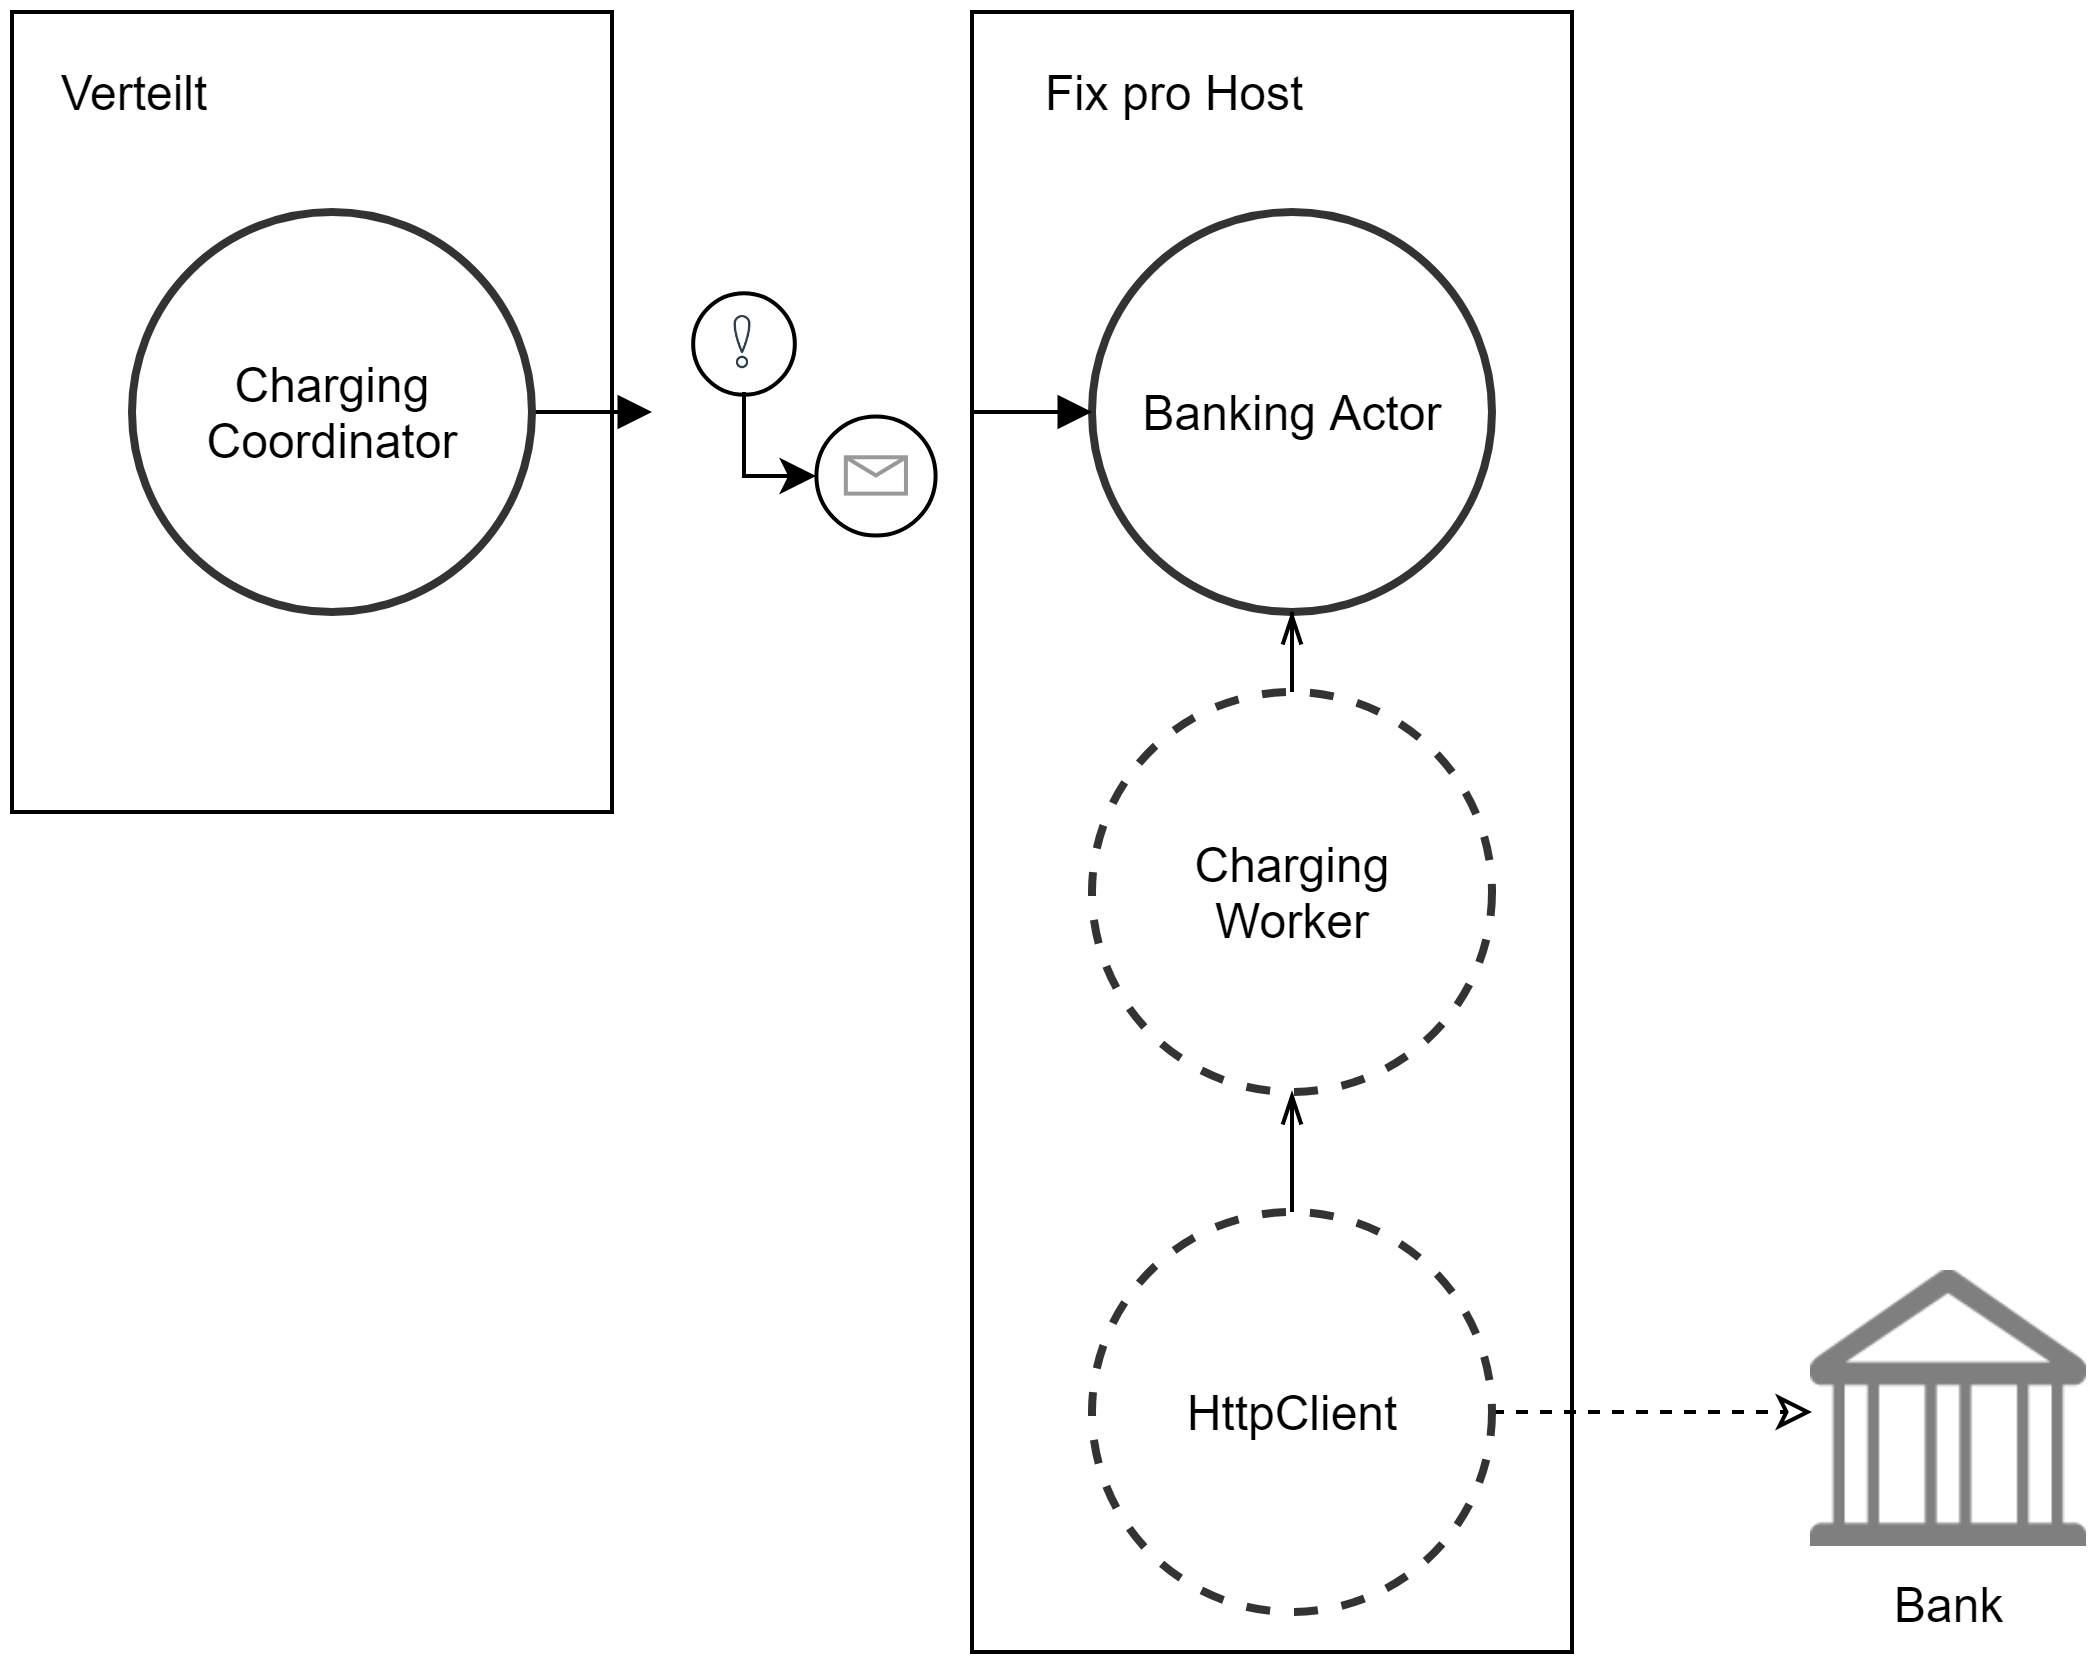
\includegraphics[width=0.65\linewidth]{gfx/implementation/ChargingCoordinatorSample}
    \caption{Modelierung des verteilten Buchungskoordinator, welcher eine nicht verteilten Actor für Anfragen an Banken verwendet}
    \label{fig:implementation:ChargingCoordinatorSample}
\end{figure}


